\begin{frame}
\frametitle{Avionics}
\begin{center}
Automatic Dependent Surveillance -- Broadcast
\par
ADS-B
\end{center}
\end{frame}

\begin{frame}
\frametitle{ADS-B}
\begin{center}
ADS-B is an electronic system aboard aircraft that broadcasts a radio signal containing certain information about that aircraft, to:
\begin{itemize}
\item other aircraft
\item air traffic control on the ground
\item anyone else who chooses to receive the signal
\end{itemize}
\end{center}
\end{frame}

\begin{frame}
\frametitle{ADS-B}
\begin{block}{ADS-B}
\begin{itemize}
\item The ICAO identifier for the airframe.
\item The flight identifier e.g. aircraft callsign.
\item Aircraft position.
\item The integrity of the position report e.g. GPS accuracy.
\item Altitude as a function of barometric pressure.
\item Altitude as a function of GPS.
\item Rate of climb/descent.
\item Aircraft ground track.
\item Aircraft ground speed.
\item Any emergency indicators.
\end{itemize}
\end{block}
\end{frame}

\begin{frame}
\frametitle{ADS-B}
\begin{block}{ADS-B receive}
\begin{itemize}
\item<1-> We can receive ADS-B signals on 1090MHz with a SDR.
\item<2-> Raspberry-pi, DVB Tuner, 1090MHz antenna.
\end{itemize}
\end{block}
\end{frame}

\begin{frame}
\frametitle{ADS-B}
\begin{block}{You are no doubt wondering}
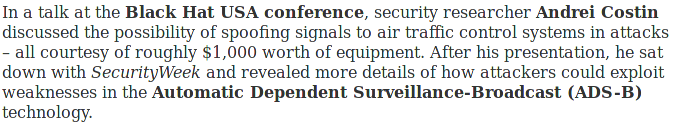
\includegraphics[height=0.18\textheight]{image/adsb-security.png}
\end{block}
Yes the absence of security in ADS-B has been demonstrated.
\end{frame}

\begin{frame}
\frametitle{Portable ADS-B receiver hardware}
\begin{block}{Portable ADS-B receiver hardware}
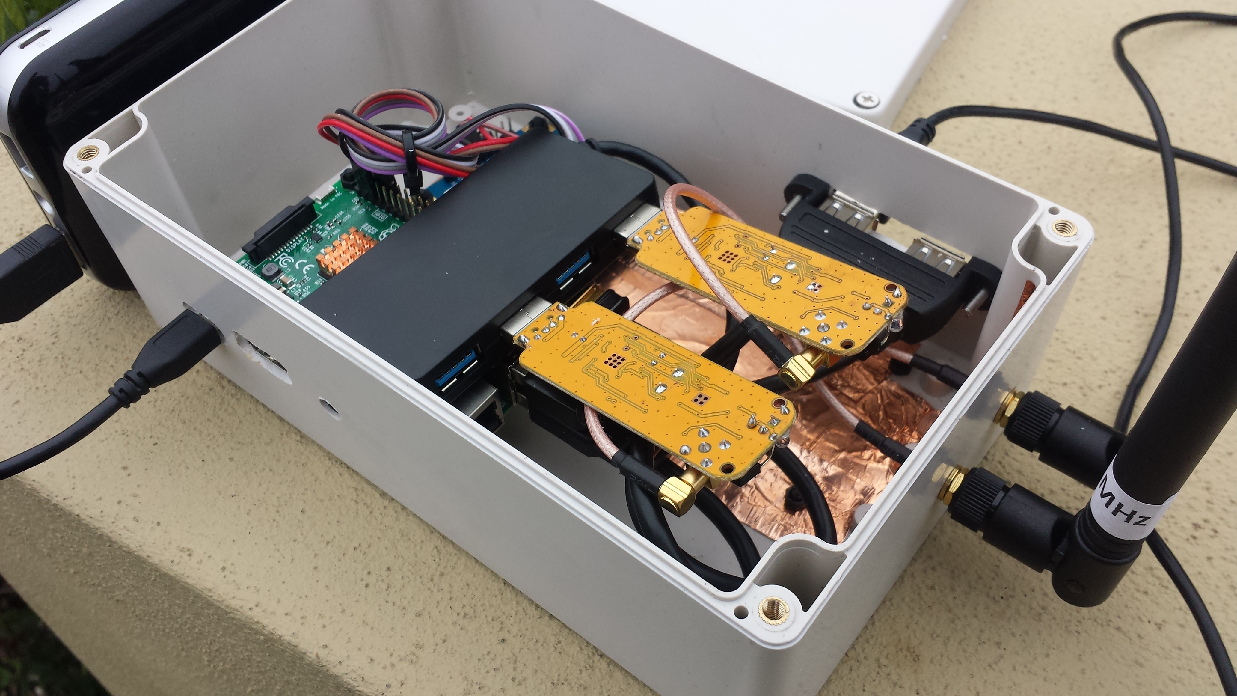
\includegraphics[height=0.5\textheight]{image/adsb-hardware.png}
\end{block}
\end{frame}

\begin{frame}
\frametitle{Portable ADS-B receiver hardware}
\begin{block}{RTL2832U Digital DVB-T (x2)}
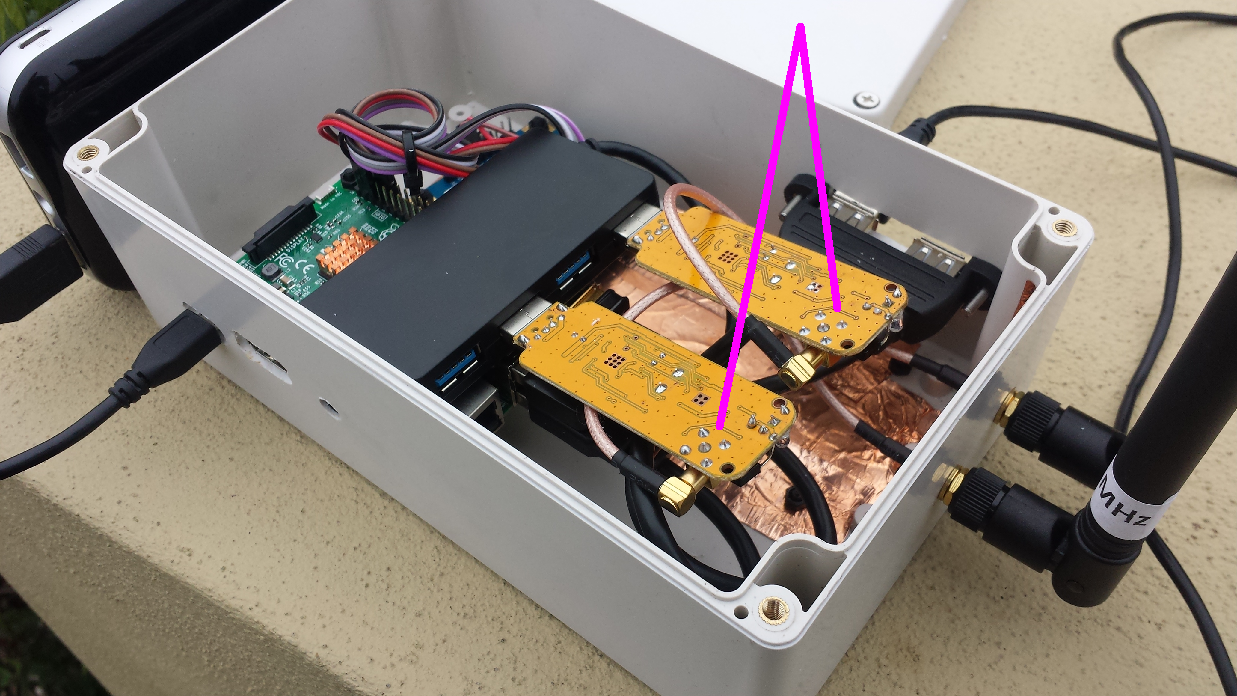
\includegraphics[height=0.5\textheight]{image/adsb-hardware-dvb.png}

RTL2832U Digital DVB-T to receive 1090MHz
\end{block}
\end{frame}

\begin{frame}
\frametitle{Portable ADS-B receiver hardware}
\begin{block}{Dual 1090MHz Antennae}
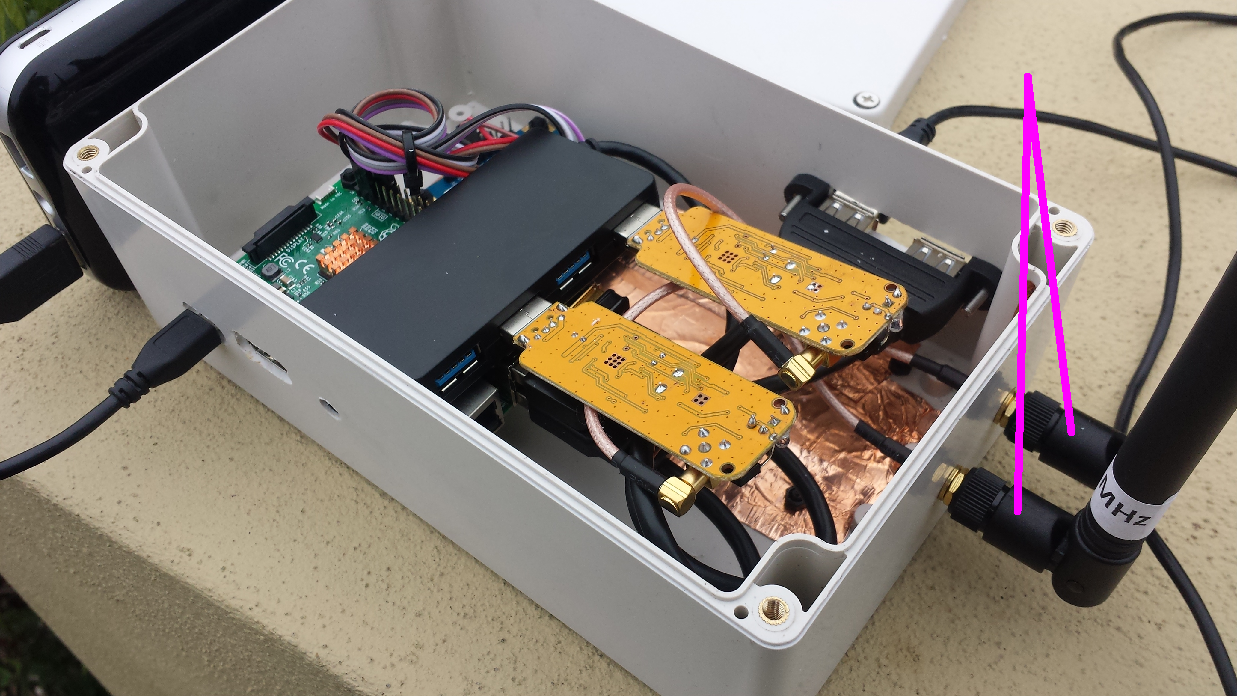
\includegraphics[height=0.5\textheight]{image/adsb-hardware-antennae.png}
\end{block}
\end{frame}

\begin{frame}
\frametitle{Portable ADS-B receiver hardware}
\begin{block}{VK-162 GPS}
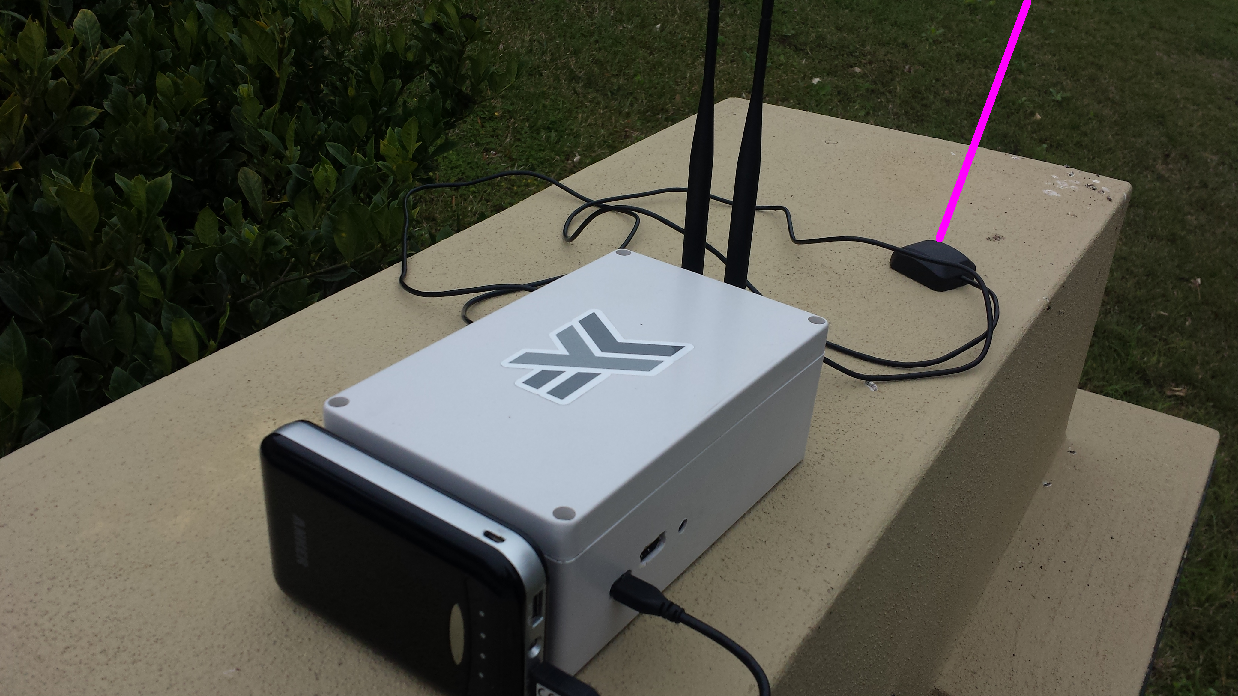
\includegraphics[height=0.5\textheight]{image/adsb-hardware-vk162.png}
\begin{itemize}
\item External GPS antenna
\item Provides track, ground speed
\end{itemize}
\end{block}
\end{frame}

\begin{frame}
\frametitle{Portable ADS-B receiver hardware}
\begin{block}{RY835AI}
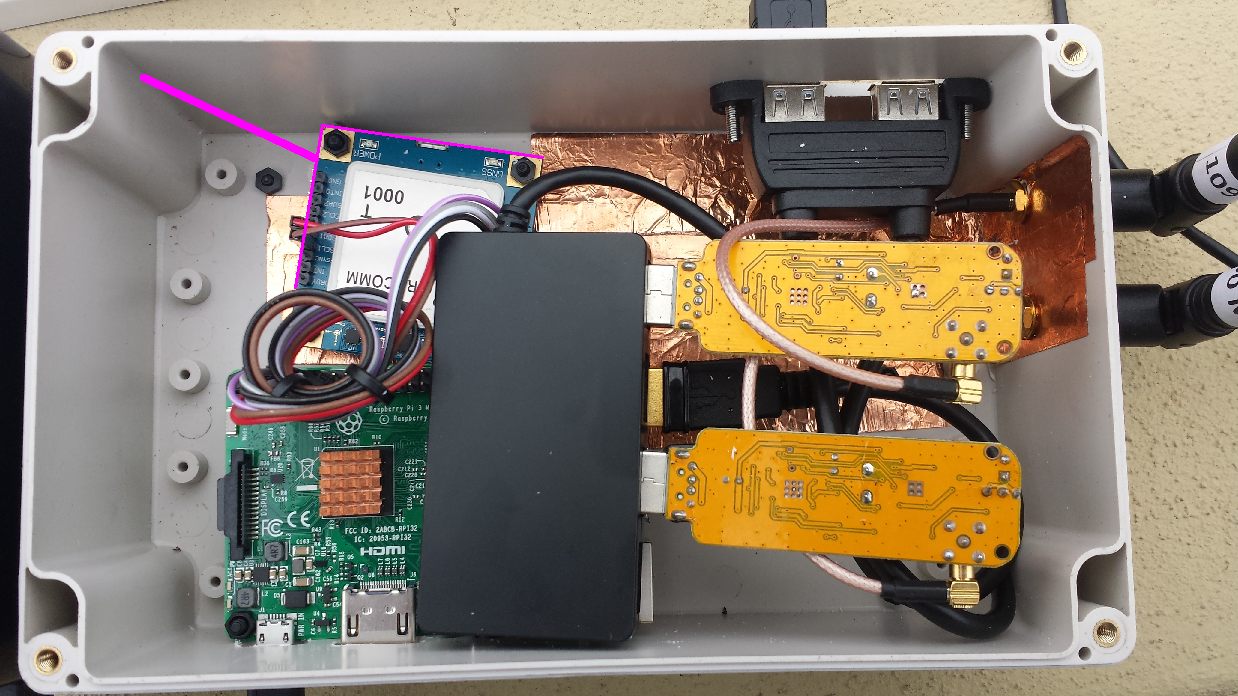
\includegraphics[height=0.5\textheight]{image/adsb-hardware-ry835ai.png}

Gyrometer providing roll, pitch and yaw
\end{block}
\end{frame}

\begin{frame}
\frametitle{Portable ADS-B receiver software}
\begin{block}{Stratux GPS/AHRS web}
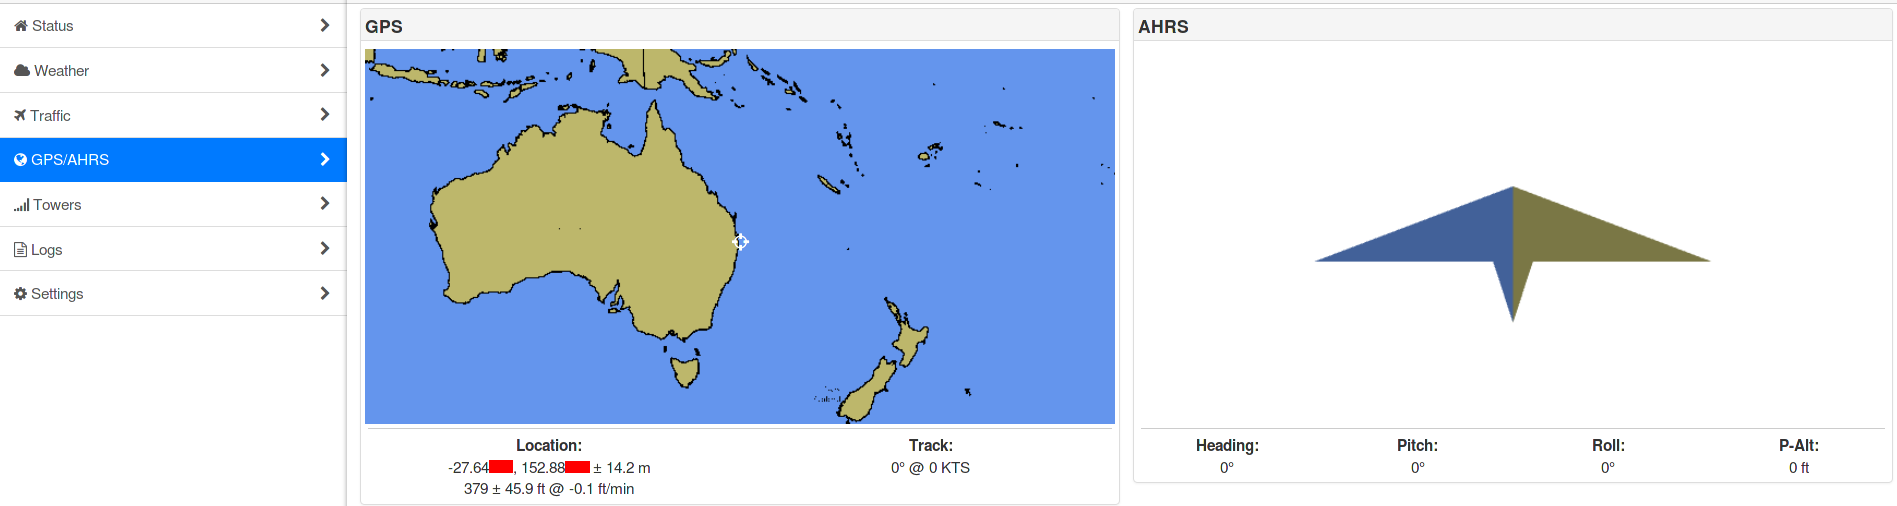
\includegraphics[height=0.32\textheight]{image/stratux-gps-ahrs-web.png}
\end{block}
\end{frame}

\begin{frame}
\frametitle{Portable ADS-B receiver software}
\begin{block}{Stratux Traffic web}
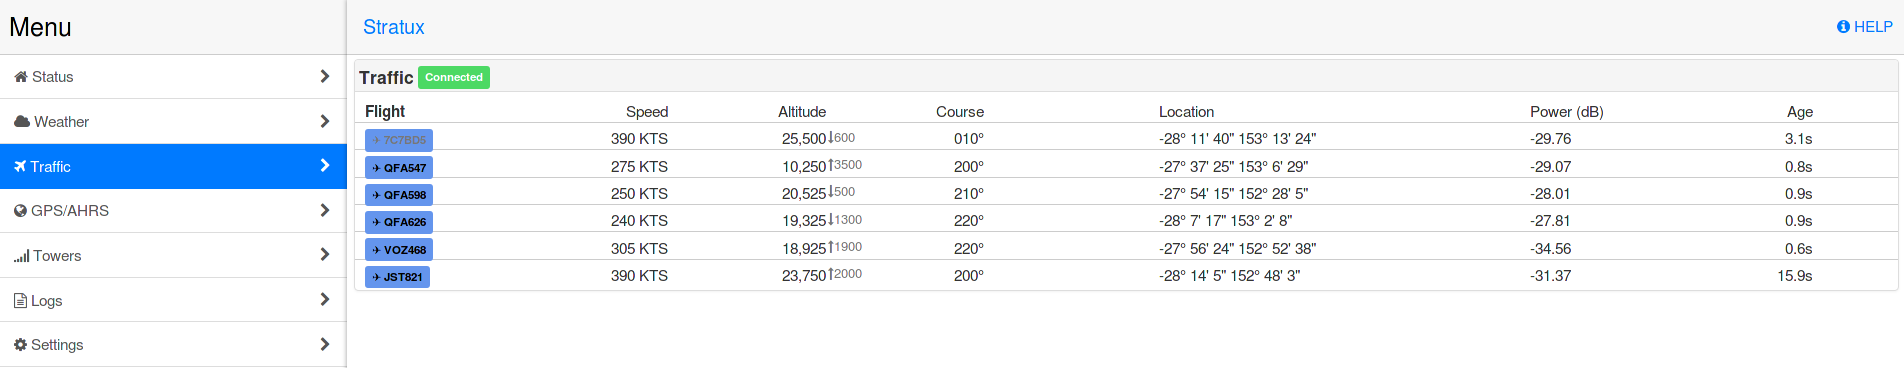
\includegraphics[height=0.23\textheight]{image/stratux-traffic-web.png}
\end{block}
\end{frame}

\begin{frame}
\frametitle{Portable ADS-B receiver software}
\begin{block}{Traffic record data type}
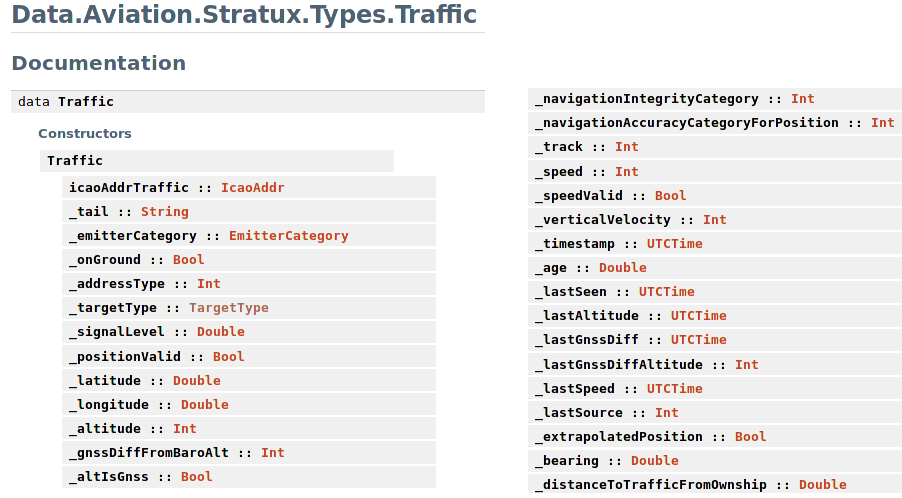
\includegraphics[height=0.6\textheight]{image/stratux-traffic-record.png}
\end{block}
\end{frame}

\begin{frame}
\frametitle{Portable ADS-B receiver software}
\begin{block}{Situation record data type}
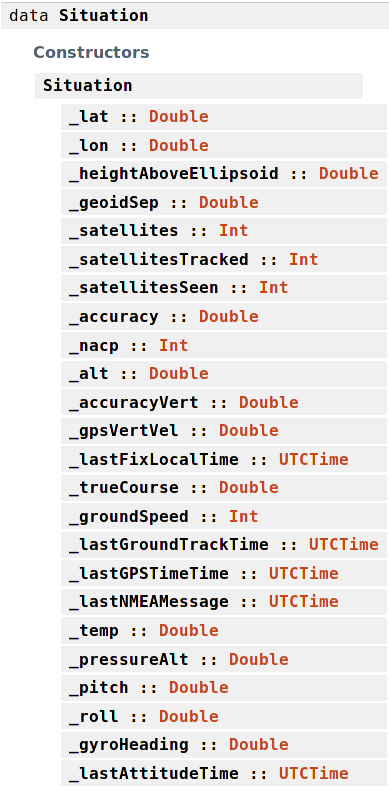
\includegraphics[height=0.6\textheight]{image/stratux-situation-record.png}
\end{block}
\end{frame}

\begin{frame}
\frametitle{Portable ADS-B receiver software}
\begin{center}
Let's code!
\end{center}
\end{frame}
